\documentclass[11pt]{article}

\usepackage[utf8]{inputenc}
\usepackage[a4paper]{geometry}
\usepackage{graphicx}
\usepackage{enumitem}
\usepackage{mdframed}
\usepackage{caption}
\usepackage{xcolor}
\usepackage[english]{babel}
\usepackage{minted}
\usepackage{longtable}
\usepackage{hyperref}

\graphicspath{ {./figures/} }

\hypersetup {
    colorlinks,
    linkcolor={red!50!black},
    citecolor={blue!50!black},
    urlcolor={blue!80!black}
}

\setlength{\parindent}{0em}
\setlength{\parskip}{0.5em}

\title{ILP Coursework 2 Report}
\author{Angus Stewart (s1902147)}
\date{December 2020}

\begin{document}

\maketitle
\thispagestyle{empty}

\newpage

\tableofcontents

%%%
\newpage
\newgeometry{left=1.5cm, right=1.5cm, top=2cm, bottom=2cm}
%%%

\section{Software Architecture}
When reading the coursework specification, it was clear that there were two distinct components to this practical. The first being the \textbf{web server} and the second being the \textbf{drone}. For this reason, I decided to create two sub-packages within my \texttt{aqmaps} package to contain all the classes related to each component. My \texttt{App.java} puts the pieces together to form the final application (e.g. by dealing with the command-line inputs and calling the appropriate public methods of objects of the classes defined in the sub-packages).

The overall structure is shown in Figure \ref{fig:uml}. The links between the classes indicate a direct relationship (e.g a method of an object of one class requires an object of another). Self-links are not included.
\begin{figure}[h]
    \centering
    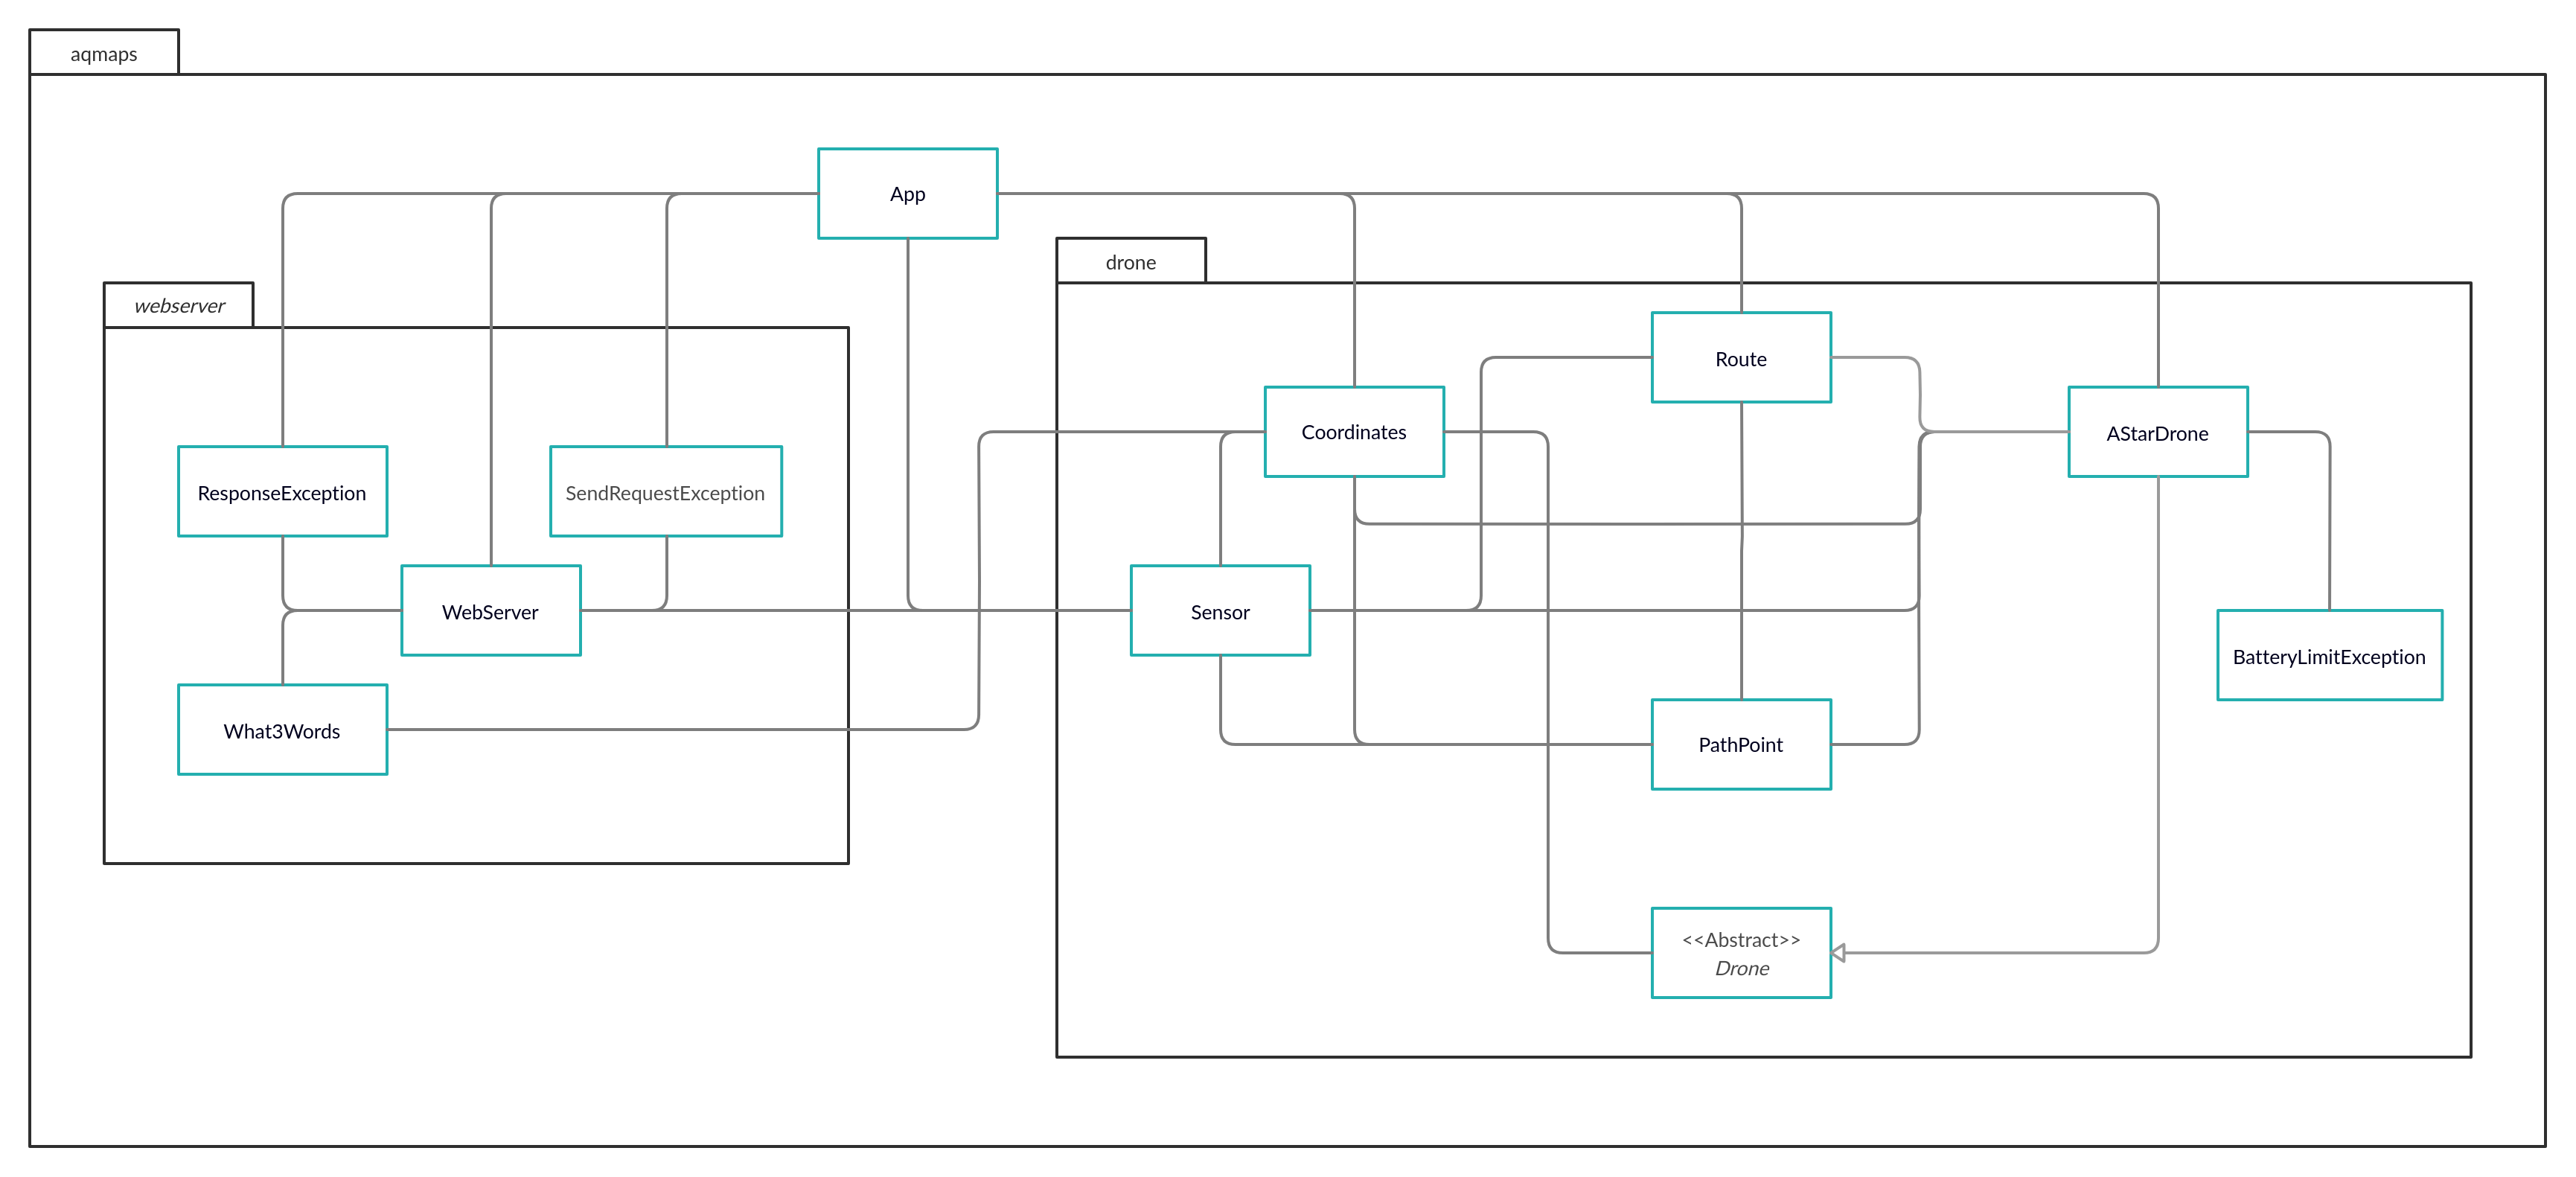
\includegraphics[width=\textwidth]{class-diagram}
    \captionof{figure}{Class diagram of \texttt{aqmaps}}
    \label{fig:uml}
\end{figure}

\subsection{\texttt{webserver}}
The \texttt{webserver} sub-package deals exclusively with \textbf{obtaining information from the web server}. The sub-package contains 4 classes related to this task:
\begin{enumerate}[topsep=0pt, itemsep=0pt]
    \item \texttt{WebServer}
    \item \texttt{What3Words}
    \item \texttt{SendRequestException}
    \item \texttt{ResponseException}
\end{enumerate}

The \texttt{WebServer} is the main class in this package and provides a layer of abstraction over all communication to the web server. It made sense to create a web server class because the web server is an standalone entity within our system. The \texttt{WebServer} class models this and provides some useful methods for retrieving data from the server. The other three classes support the main \texttt{WebServer} class. The \texttt{What3Words} class is used to store the JSON information obtained from the \texttt{words/} directory on the web server as a Java object. It is required to parse the JSON with \texttt{gson}. We also use the \texttt{Sensor} class from the \texttt{drone} sub-package when obtaining sensor information from the web server. The reason this class was included in the \texttt{drone} sub-package was because it did not make much sense to store a class that represents a physical sensor in a package dedicated to dealing with a web server. It made more sense to include it in the drone package where the drone is modelled due to the close relationship that these two objects have in this practical. A similar reasoning applies to \texttt{Coordinates} (described more in the next section).

The other two classes (\texttt{SendRequestException} and \texttt{ResponseException}) were created to abstract over the specific exceptions that can occur when communicating with the web server. The \texttt{SendRequestException} abstracts over the exceptions related to the creation and sending of the HTTP request (e.g. if an invalid URI was provided). The \texttt{ResponseException} abstracts over the exceptions relating to the HTTP reponse from the web server (e.g. if a 404 response was returned). This provides a cleaner interface to the \texttt{webserver} class as it abstracts away unnecessary complexity and verbosity.

\subsection{\texttt{drone}}
This sub-package consists of a set of classes related to the \textbf{drone and its internal representation of the world}. In other words, these classes together model the problem detailed in the specification of finding, and presenting, the flight path of a drone around a geographical area with no-fly-zones, in order to collect readings from a set of sensors. This may seem like a lot of disparate ideas, but they are very closely related.

There are 7 classes in this sub-package:
\begin{enumerate}[topsep=0pt, itemsep=0pt]
    \item \texttt{Drone}
    \item \texttt{AStarDrone}
    \item \texttt{Sensor}
    \item \texttt{Route}
    \item \texttt{PathPoint}
    \item \texttt{Coordinates}
    \item \texttt{BatteryLimitException}
\end{enumerate}

The \texttt{Drone} class models the \textbf{physical properties that affect the drone}. For example, it defines the method \texttt{move} which models how the drone moves and \texttt{getDistance} which defines the measure of distance between two points in the real world. It also has attributes that describe the confinement area and methods for processing the no-fly-zones. All together, this class models the relationship between the drone and the physical world as detailed in the specification. For this reason, the \texttt{Drone} class is abstract as instantiating it on its own is doesn't make much sense.

This brings us to the \texttt{AStarDrone} class which models the \textbf{behaviour of the drone}. It inherits from the \texttt{Drone} class to understand the physical world, then it uses its own methods to navigated within that world. This class is where the drone control algorithm (detailed in section \ref{drone_alg}) is implemented. It receives the initial starting conditions of the world (i.e sensors, starting position, and no-fly-zones) to calculate an appropriate route which visits all the sensors and returns to the original starting position.

\begin{mdframed}
In my original implementation, I only had one \texttt{GreedyDrone} class which combined both \texttt{Drone} and \texttt{AStarDrone} (but used a greedy approach instead of an A* based approach). I then decided to create a new drone control algorithm based on the A* search algorithm as the greedy approach I was using was giving me some problems. I soon noticed that some functions and attributes were being duplicated in both the \texttt{GreedyDrone} class and the then newly created \texttt{AStarDrone} class. This was the original motivation behind creating a parent class; to `pull out' this shared implementation to make the code more maintainable (DRY!). The abstract nature of the parent class became apparent when, upon closer inspection, I realized that the code I was pulling out reflected the rules of the physical world in which the drone was operating under as described in the specification (e.g distance of a single move of the drone, the distance measure, the confinement area, etc).
\end{mdframed}

The \texttt{Route} object is the third main class within this sub-package. This class arose due to a strong emphasis that the specification placed on the route of the drone as a GeoJSON map and as a flightpath in txt format. I felt that modelling the route itself was appropriate as the GeoJSON map and the flightpath were simply different representations of the same underlying concept. This class provides convenient methods to obtain both the flightpath and the GeoJSON map of the route as \texttt{.txt} and \texttt{.geojson} files respectively.

The two classes \texttt{Coordinates} and \texttt{PathPoint} both represent important concepts in the drone's internal representation of the world. The \texttt{Coordinates} class represents the latitude and longitude values of a position in the world as described in the specification. This abstraction is incredibly useful for representing the position of objects such as the sensors or the drone itself. The \texttt{PathPoint} object represents a single movement of the drone from one position to another. This class is used to represent each line of the flightpath txt file. It is also used within the drone to represent the global route as a sequence of drone movements and in the drone control algorithm as a way to represent the different possible movement options that the drone has at each particular position.

Finally, the \texttt{BatteryLimitException} class is used to represent the event where the route to a sensor generated by the drone control algorithm is longer than what the battery of the drone allows. By raising this exception the control algorithm can react and create a contingency plan (e.g by returning to the starting position). This class is not essential but proved to be convenient when implementing the control algorithm.

\section{Drone Control Algorithm} \label{drone_alg}
The specification describes a similar problem to the well known \href{https://en.wikipedia.org/wiki/Travelling\_salesman\_problem}{travelling salesman problem} (TSP) where we look to visit each sensor and return to the starting position. It is not exactly the same problem as the path to each sensor is not a single link but rather a series of restricted movements. Hence, the combination of the travelling salesman problem being NP-complete and the movements of the drone made the complexity of the problem very apparent from the beginning.

Knowing that finding an algorithm that would solve the entire path planning problem optimally would not be feasible, I broke the problem into two sub-problems. The first is the order in which the drone visits the sensors and the second is finding the sequence of valid moves to get from one coordinate position to another.

With these two components, we can find the entire route:
\begin{enumerate}[topsep=0pt, itemsep=0pt]
    \item Get the next \textbf{unvisited} sensor given the current position of the drone
    \item Find the route to the sensor
    \begin{enumerate}[topsep=0pt, itemsep=0pt]
        \item If enough battery, move the drone along the route and mark the sensor as visited
        \item Otherwise, skip to step 4
    \end{enumerate}
    \item Go to step 1 until all sensors have been visited
    \item Find the route back to the start given the current position. If not enough battery to complete the entire route, follow the route until we run out of battery to return as close to the start as possible.
\end{enumerate}


\begin{figure}[h]
    \centering
    \begin{minipage}{0.5\textwidth}
        \centering
        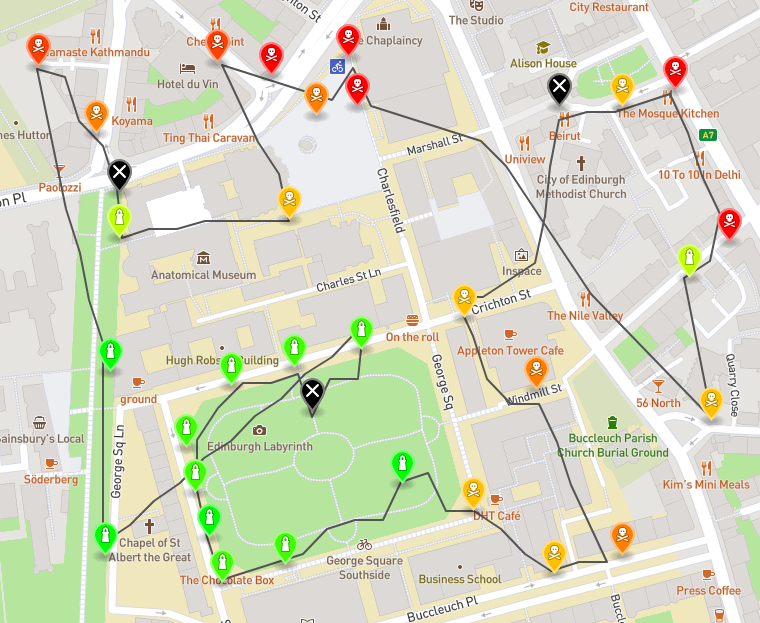
\includegraphics[width=0.95\textwidth, height=16em]{25-10-2021}
        \captionof{figure}{25th of October 2021}
        \label{fig:example1}
    \end{minipage}%
    \begin{minipage}{0.5\textwidth}
        \centering
        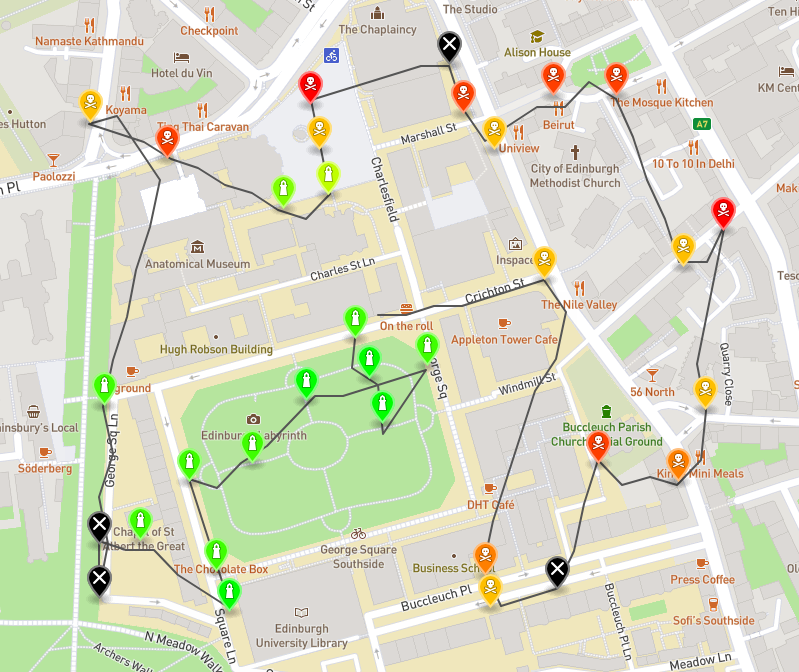
\includegraphics[width=0.95\textwidth, height=16em]{26-12-2021}
        \captionof{figure}{26th of December 2021}
        \label{fig:example2}
    \end{minipage}
\end{figure}

\subsection{Ordering of the Sensors}
The first problem is determining the order in which the drone should visit the sensors. To keep things simple, I chose a greedy approach, and this is what the drone uses in the implementation. The algorithm calculates the straight-line distance between a given coordinate position (e.g. current position of the drone) and the coordinates of a list of sensors (e.g. list of unvisited sensors) and returns the closest sensor.

Although this algorithm is simple and runs very quickly (linear in the number of sensors), it is unlikely to produce an optimal sequence of sensors to visit. We can see this with Figure \ref{fig:example1} where the drone has to travel long distances across the map to visit the next sensor when a different ordering would have prevented this from happening. In addition, it does not take into account the no-fly-zones of the map and how this affects the distances between sensors. But given the TSP nature of this problem, obtaining good solutions requires significant effort in implementing complex algorithms. Hence, I believe this greedy algorithm is a good starting point due to its balance of simplicity and performance.

It is worth noting that the drone only looks for the next sensor and does not pre-compute the order of all sensors. This decision was taken because the drone does not necessarily reach the exact coordinates of the target sensor and hence pre-computing everything from the beginning would be inaccurate.

\subsection{Routing to the Next Position}
Given the current position of the drone and the target position (e.g coordinates of the next sensor or of the starting position), we must calculate a valid route between the two points. Note that we do not need to end up \textbf{at} the target position, just within a certain distance from it (e.g 0.0002 for sensors).

This can be thought of as a tree search problem. The tree represents all possible sequences of moves (represented by the edges of the tree) that the drone is allowed to make, and the nodes represents coordinate positions with the root being the current position of the drone. Note that the branching factor for this tree is 36 (though it may be less if the movement of the drone is restricted e.g due to being near no-fly-zones).

In my implementation, I use a modified A* search algorithm to find the path down the tree to a node that is within range of our target position. The algorithm consists of two lists: \texttt{closedPathPoints}, which stores all the nodes that we have visited (expanded) and \texttt{openPathPoints}, which stores all the nodes that we have yet to visit but whose parents have been visited.
\begin{enumerate}[topsep=0pt, itemsep=0pt]
  \item We begin with the root node. 'Expand' it to generate all \textbf{valid} children nodes \footnote{To check if a child node is valid, we take the line segment formed by the parent node and the child node and see if it intersects (using the \texttt{java.awt.geom} package) with an edge of the drone confinement area or no-fly-zones. If it does, it is invalid.}. These child nodes represent positions the drone can move to in one step that does not violate any of the rules (e.g regarding no-fly-zones).
  \begin{enumerate}[topsep=0pt, itemsep=0pt]
      \item Each child node gets assigned a \texttt{distanceScore} (among other attributes such as \texttt{prev}) which is the sum of the travelled distance from the root to the current node and the straight-line distance from the current node to the target position.
      \item We then select 5 of the child nodes with the smallest \texttt{distanceScore}. We do this to reduce the time complexity of the algorithm as using all child nodes would cause the algorithm to run slowly.
  \end{enumerate}
  
  \item Add the 5 nodes to \texttt{openPathPoints} and add the root to \texttt{closedPathPoints}
  
  \item Select the node from \texttt{openPathPoints} with the lowest \texttt{distanceScore} and remove it from the list. If in range of the target position, skip to step 6, otherwise expand it as per step 1.
  
  \item Before adding each of the 5 nodes to \texttt{openPathPoints}, we do two checks:
  \begin{enumerate}[topsep=0pt, itemsep=0pt]
      \item If their coordinates match with a node already in \texttt{openPathPoints}, we look to see if it has a smaller \texttt{distanceScore}. If it does, we add the new node and remove the old one. Otherwise, we discard the new node.
      \item If the node was not added to \texttt{openPathPoints} or discarded in part (a), check to see if the coordinates match with a node already in \texttt{closedPathPoints}. If it does, discard the node.      
    \end{enumerate}   
    
  \item Add the expanded node (from step 3) to \texttt{closedPathPoints} and go to step 3

  \item Reconstruct the route from the final node from step 3 by following \texttt{prev} (which points to the node's parent) until we reach the root.
\end{enumerate}

Notice that this algorithm will always produce a route of at least length 1 because it always expands the root node before checking if any of the nodes are within range of the target position. This is required as per the specification. However, because we do not need to move before finishing, when calculating the route back to the start we check before step 1 whether the root is within range of the target position.

This algorithm has the advantage that it can handle no-fly-zones without much modification (we just don't generate the child nodes that cross the no-fly-zones). This contrasts with my original algorithm that used a greedy approach which would get `stuck' oscillating between two nodes if the target position was on the other side of a no-fly-zone. This is because unlike the A* search algorithm, the greedy algorithm did not take into account the distance from the root node. However, the time complexity of the A* algorithm is not as good (hence step 1.b) so the time the algorithm takes to find routes over larger distances become much more noticeable which puts the scalability of this algorithm into question.

It is also worth mentioning here, that although \textbf{the algorithm is the same}, in the actual implementation we use \texttt{PathPoint} objects, which represent the movement of the drone and hence would correspond to the edges of the tree, rather than nodes as described above. However, \texttt{PathPoint} stores the child node in \texttt{endPos} (and its parent in \texttt{startPos}) and attributes such as \texttt{distanceScore} correspond to the position of \texttt{endPos}, so the implementation details of the algorithm is very similar.

\section{Class Documentation}

\subsection{\texttt{uk.ac.ed.inf.aqmaps}}


\begin{center}
    \phantomsection
    \addcontentsline{toc}{subsubsection}{\texttt{App}}
    \begin{tabular}{ |p{2em} c c| } \hline
        \multicolumn{3}{ |c| }{\texttt{App}} \\
    
        \hline \hline
    
        & & \\
        
        \multicolumn{3}{|l|}{
            \begin{minipage}{{\textwidth}}
                This class encapsulates the application as described in the specification.
            \end{minipage} 
        } \\
        
        & & \\
    
        \multicolumn{3}{|l|}{
            \begin{minipage}{{0.9\textwidth}}
                \mint[fontsize=\small]{java}|public static void main(String[] args)|
                \vspace{-0.5em}
            \end{minipage}
        } \\
    
        & \begin{minipage}{0.9\textwidth}
            This method is the main entry point into the application. \\
        
            It is responsible for pulling in the different components defined in the \texttt{drone} and \texttt{webserver} sub-packages to provide the expected top-level behaviour of the application (i.e. process the command-line inputs, get information from the web server, calculate the route of the drone and save this information to the two output files). \\
        
            Parameters:
            \begin{itemize}[label={}, topsep=0pt, itemsep=0pt]
                \item \texttt{args}: command-line arguments as defined in the specification
            \end{itemize}
        \end{minipage} & \\ & & \\ \hline
    \end{tabular}
\end{center}



\subsection{\texttt{uk.ac.ed.inf.aqmaps.webserver}}


\begin{center}
    \phantomsection
    \addcontentsline{toc}{subsubsection}{\texttt{WebServer}}
    \begin{longtable}{ |p{2em} c c| } \hline
    \multicolumn{3}{ |c| }{\texttt{WebServer}} \\
    
    \hline \hline
    
    & & \\
    
    \multicolumn{3}{|l|}{
        \begin{minipage}{{\textwidth}}
            This class encapsulates methods relating to communication with the web server. The class attributes are \texttt{client} which stores the \texttt{HttpClient} that sends the HTTP GET requests (this is static because we want to prevent multiple instances of the client being created), \texttt{noFlyZonePath} which stores the file path to the \texttt{geojson} file for the no-fly-zones, \texttt{protocol} which stores the protocol to use in the URI (e.g. http), \texttt{host} which stores the host name of the web server and \texttt{port} which stores the port number to access.
        \end{minipage} 
    } \\
    
    & & \\
    
    \multicolumn{3}{|l|}{
        \begin{minipage}{{0.9\textwidth}}
            \mint[fontsize=\small]{java}|public class WebServer(String protocol, String host, String port)|
            \vspace{-0.5em}
        \end{minipage}
    } \\
    
    & \begin{minipage}{0.9\textwidth}
        Creates and initializes a \texttt{WebServer} object that sends requests to the specified web server.  \\
        
        Parameters:
        \begin{itemize}[label={}, topsep=0pt, itemsep=0pt]
            \item \texttt{protocol}: the protocol to use to send requests (e.g \texttt{http})
            \item \texttt{host}: the host name of the server to send requests to (e.g \texttt{localhost})
            \item \texttt{port}: the port number to connect to (e.g \texttt{80})
        \end{itemize}
    \end{minipage} & \\

    %%%%%%%%%%%
    & & \\
    %%%%%%%%%%%
    
    \multicolumn{3}{|l|}{
        \begin{minipage}{{0.9\textwidth}}
            \mint[fontsize=\small]{java}|public ArrayList<Sensor> getSensorsWithCoordinates(String year, String month, String day)|
            \vspace{-0.5em}
        \end{minipage}
    } \\
    
    & \begin{minipage}{0.9\textwidth}
        This method returns a list of \texttt{Sensor} objects for the specified date \textbf{with} coordinate information pre-populated. This is a convenience function built on top of \texttt{getSensors} and \texttt{getWhat3WordsDetails}. This method will send multiple HTTP requests, one for the relevant \texttt{air-quality-data.json} file and one for each sensor to get its coordinate position. \\
        
        Parameters:
        \begin{itemize}[label={}, topsep=0pt, itemsep=0pt]
            \item \texttt{year}: year of the desired date (must be 4 digits e.g. ``2020")
            \item \texttt{month}: month of the desired date (must be 2 digits e.g. ``02")
            \item \texttt{day}: day of the desired date (must be 2 digits e.g. ``02")
        \end{itemize}
        
        \vspace{1em}
        
        Throws:
        \begin{itemize}[label={}, topsep=0pt, itemsep=0pt]
            \item \texttt{SendRequestException}: if another exception occurs while creating or sending the request
            \item \texttt{ResponseException}: if the response object is \texttt{null} or the response code is not 200
        \end{itemize}
    \end{minipage} & \\
    
    %%%%%%%%%%%
    & & \\
    %%%%%%%%%%%    
    
    \multicolumn{3}{|l|}{
        \begin{minipage}{{0.9\textwidth}}
            \mint[fontsize=\small]{java}|public ArrayList<Sensor> getSensors(String year, String month, String day)|
            \vspace{-0.5em}
        \end{minipage}
    } \\
    
    & \begin{minipage}{0.9\textwidth}
        This method returns a list of \texttt{Sensor} objects \textbf{without} coordinate information (i.e the \texttt{coordinates} attribute of each object is \texttt{null}). Hence, this method only sends a single request to the server to obtain the \texttt{air-quality-data.json} file for the specified date. \\
        
        Parameters:
        \begin{itemize}[label={}, topsep=0pt, itemsep=0pt]
            \item \texttt{year}: year of the desired date (must be 4 digits e.g. ``2020")
            \item \texttt{month}: month of the desired date (must be 2 digits e.g. ``02")
            \item \texttt{day}: day of the desired date (must be 2 digits e.g. ``02")
        \end{itemize}
        
        \vspace{1em}
        
        Throws:
        \begin{itemize}[label={}, topsep=0pt, itemsep=0pt]
            \item \texttt{SendRequestException}: if another exception occurs while creating or sending the request
            \item \texttt{ResponseException}: if the response object is \texttt{null} or the response code is not 200
        \end{itemize}
    \end{minipage} & \\ 
    
    %%%%%%%%%%%    
    & & \\
    %%%%%%%%%%%
    
    \multicolumn{3}{|l|}{
        \begin{minipage}{{0.9\textwidth}}
            \mint[fontsize=\small]{java}|public What3Words getWhat3WordsDetails(String location)|
            \vspace{-0.5em}
        \end{minipage}
    } \\
    
    & \begin{minipage}{0.9\textwidth}
        This method returns a \texttt{What3Words} object for the specified What3Words string. This is useful as the resulting object contains the coordinate position of the sensor at the What3Words location. Only one request to the server is made to get the \texttt{details.json} file of the given location string.\\
        
        Parameters:
        \begin{itemize}[label={}, topsep=0pt, itemsep=0pt]
            \item \texttt{location}: the What3Words location (e.g. ``\texttt{hurt.green.filer}")
        \end{itemize}
        
        \vspace{1em}
        
        Throws:
        \begin{itemize}[label={}, topsep=0pt, itemsep=0pt]
            \item \texttt{SendRequestException}: if another exception occurs while creating or sending the request
            \item \texttt{ResponseException}: if the response object is \texttt{null} or the response code is not 200
        \end{itemize}
    \end{minipage} & \\
    
    %%%%%%%%%%%    
    & & \\
    %%%%%%%%%%%
    
    \multicolumn{3}{|l|}{
        \begin{minipage}{{0.9\textwidth}}
            \mint[fontsize=\small]{java}|public FeatureCollection getNoFlyZones()|
            \vspace{-0.5em}
        \end{minipage}
    } \\
    
    & \begin{minipage}{0.9\textwidth}
        This method returns the no-fly-zone information stored in \texttt{buildings/no-fly-zones.geojson} on the web server as a \texttt{FeatureCollection}. \\
        
        Throws:
        \begin{itemize}[label={}, topsep=0pt, itemsep=0pt]
            \item \texttt{SendRequestException}: if another exception occurs while creating or sending the request
            \item \texttt{ResponseException}: if the response object is \texttt{null} or the response code is not 200
        \end{itemize}
    \end{minipage} & \\ 
    
    %%%%%%%%%%%    
    & & \\
    %%%%%%%%%%%    
    
    \multicolumn{3}{|l|}{
        \begin{minipage}{{0.9\textwidth}}
            \mint[fontsize=\small]{java}|private HttpResponse<String> sendRequest(String filePath)|
            \vspace{-0.5em}
        \end{minipage}
    } \\
    
    & \begin{minipage}{0.9\textwidth}
        This method is a utility function that sends a HTTP GET request to the web server asking for the resource at the given file path and returns the \texttt{HttpResponse<String>} object if the status code is 200, otherwise an exception is thrown. \\
        
        Parameters:
        \begin{itemize}[label={}, topsep=0pt, itemsep=0pt]
            \item \texttt{filepath}: the path to the desired resource on the web server
        \end{itemize}
        
        \vspace{1em}
        
        Throws:
        \begin{itemize}[label={}, topsep=0pt, itemsep=0pt]
            \item \texttt{SendRequestException}: if another exception occurs while creating or sending the request
            \item \texttt{ResponseException}: if the response object is \texttt{null} or the response code is not 200
        \end{itemize}
    \end{minipage} & \\     
    
    & & \\ \hline
\end{longtable}
\end{center}


\vspace{-2.5em}


\begin{center}
    \phantomsection
    \addcontentsline{toc}{subsubsection}{\texttt{What3Words}}
    \begin{tabular}{ |p{2em} c c| } \hline
        \multicolumn{3}{ |c| }{\texttt{What3Words}} \\
    
        \hline \hline
        
        & & \\
    
        \multicolumn{3}{|l|}{
            \begin{minipage}{{\textwidth}}
                This class encapsulates all the information for a particular What3Words location string stored on the web server as described in the specification. It has no methods, just used to encapsulate the information.
            \end{minipage} 
        } \\
    
        & & \\ \hline
   \end{tabular}
\end{center}


\vspace{-1.5em}


\begin{center}
    \phantomsection
    \addcontentsline{toc}{subsubsection}{\texttt{SendRequestException}}
    \begin{tabular}{ |p{2em} c c| } \hline
        \multicolumn{3}{ |c| }{\texttt{SendRequestException}} \\
    
        \hline \hline
        
        & & \\
    
        \multicolumn{3}{|l|}{
            \begin{minipage}{{\textwidth}}
                This class provides a layer of abstraction over all exceptions that relate to the creation and sending of a HTTP request to the target web server.
            \end{minipage} 
        } \\
    
        & & \\
    
        \multicolumn{3}{|l|}{
            \begin{minipage}{{0.9\textwidth}}
                \mint[fontsize=\small]{java}|public SendRequestException(String message)|
                \vspace{-0.5em}
            \end{minipage}
        } \\
    
        & \begin{minipage}{0.9\textwidth}
            Creates and initializes a \texttt{SendRequestException} object with the provided message. \\
        
            Parameters:
            \begin{itemize}[label={}, topsep=0pt, itemsep=0pt]
                \item \texttt{message}: the message to be shown when the exception is thrown
            \end{itemize}
        \end{minipage} & \\ & & \\ \hline
    \end{tabular}
\end{center}



\vspace{-1.5em}



\begin{center}
    \phantomsection
    \addcontentsline{toc}{subsubsection}{\texttt{ResponseException}}
    \begin{tabular}{ |p{2em} c c| } \hline
        \multicolumn{3}{ |c| }{\texttt{ResponseException}} \\
    
        \hline \hline
        
        & & \\
    
        \multicolumn{3}{|l|}{
            \begin{minipage}{{\textwidth}}
                This class provides a layer of abstraction over all exceptions that relate to the HTTP response (or lack thereof) from the target web server.
            \end{minipage} 
        } \\
    
        & & \\
    
        \multicolumn{3}{|l|}{
            \begin{minipage}{{0.9\textwidth}}
                \mint[fontsize=\small]{java}|public ResponseException(String message)|
                \vspace{-0.5em}
            \end{minipage}
        } \\
    
        & \begin{minipage}{0.9\textwidth}
            Creates and initializes a \texttt{ResponseException} object with the provided message. \\
        
            Parameters:
            \begin{itemize}[label={}, topsep=0pt, itemsep=0pt]
                \item \texttt{message}: the message to be shown when the exception is thrown
            \end{itemize}
        \end{minipage} & \\ & & \\ \hline
    \end{tabular}
\end{center}


\newpage
\subsection{\texttt{uk.ac.ed.inf.aqmaps.drone}}



\begin{center}
    \phantomsection
    \addcontentsline{toc}{subsubsection}{\texttt{Drone}}
    \begin{tabular}{ |p{2em} c c| } \hline
        \multicolumn{3}{ |c| }{\texttt{Drone}} \\
    
        \hline \hline
        
        & & \\
    
        \multicolumn{3}{|l|}{
            \begin{minipage}{{\textwidth}}
                This is an \textbf{abstract class} which encapsulates methods and attributes related to the physical characteristics that affect the behaviour of the drone. It includes attributes that define the confinement area as a set of boundaries or line segments (using the \texttt{java.awt.geom} package) as well as other constants defined in the specification (i.e max number of moves, the maximum range of a sensor reading, maximum allowable distance from start position when returning and distance of each move of the drone). It also stores some non-static attributes such as \texttt{battery} which keeps track of the battery level of the drone, \texttt{boundaryLines} which stores all the line segments which the drone cannot intersect, and \texttt{noFlyZones} which stores the no-fly-zones.
            \end{minipage}  
        } \\
    
        & & \\
    
        \multicolumn{3}{|l|}{
            \begin{minipage}{{0.9\textwidth}}
                \mint[fontsize=\small]{java}|public Drone(FeatureCollection noFlyZones)|
                \vspace{-0.5em}
            \end{minipage}
        } \\
    
        & \begin{minipage}{0.9\textwidth}
            Initializes the set of line segments which the drone is not allowed to intersect while flying. \\
        
            Parameters:
            \begin{itemize}[label={}, topsep=0pt, itemsep=0pt]
                \item \texttt{noFlyZones}: the set of no-fly-zones (must be \texttt{Feature}s of type \texttt{Polygon})
            \end{itemize}
        \end{minipage} & \\
        
        & & \\
    
        \multicolumn{3}{|l|}{
            \begin{minipage}{{0.9\textwidth}}
                \mint[fontsize=\small]{java}|protected boolean isMoveValid(Coordinates start, Coordinates end)|
                \vspace{-0.5em}
            \end{minipage}
        } \\
    
        & \begin{minipage}{0.9\textwidth}
            Checks to see if the move from \texttt{start} to \texttt{end} enters a no-fly-zone or leaves the confinement area by looking to see if the move intersects any of the boundaries in \texttt{boundaryLines}. \\
        
            Parameters:
            \begin{itemize}[label={}, topsep=0pt, itemsep=0pt]
                \item \texttt{start}: the coordinate position before the move
                \item \texttt{end}: the coordinate position after the move
            \end{itemize}
        \end{minipage} & \\
        
        & & \\
    
        \multicolumn{3}{|l|}{
            \begin{minipage}{{0.9\textwidth}}
                \mint[fontsize=\small]{java}|protected static ArrayList<Line2D> getBoundaryLines(FeatureCollection noFlyZones)|
                \vspace{-0.5em}
            \end{minipage}
        } \\
    
        & \begin{minipage}{0.9\textwidth}
             Returns an array of line segments that describe the boundaries of the given no-fly-zones.\\
        
            Parameters:
            \begin{itemize}[label={}, topsep=0pt, itemsep=0pt]
                \item \texttt{noFlyZones}: the set of no-fly-zones (must be \texttt{Feature}s of type \texttt{Polygon})
            \end{itemize}
        \end{minipage} & \\
        
        & & \\
    
        \multicolumn{3}{|l|}{
            \begin{minipage}{{0.9\textwidth}}
                \mint[fontsize=\small]{java}|protected static Coordinates move(Coordinates currentPos, int direction)|
                \vspace{-0.5em}
            \end{minipage}
        } \\
    
        & \begin{minipage}{0.9\textwidth}
            Returns the position of the drone if it were to move in the given direction from the given position. \\
        
            Parameters:
            \begin{itemize}[label={}, topsep=0pt, itemsep=0pt]
                \item \texttt{currentPos}: current coordinate position of the drone
                \item \texttt{direction}: direction the drone is to move
            \end{itemize}
        \end{minipage} & \\
        
        & & \\
    
        \multicolumn{3}{|l|}{
            \begin{minipage}{{0.9\textwidth}}
                \mint[fontsize=\small]{java}|protected static double getDistance(Coordinates start, Coordinates end)|
                \vspace{-0.5em}
            \end{minipage}
        } \\
    
        & \begin{minipage}{0.9\textwidth}
            Returns the distance, in degrees, between the two specified coordinate positions. \\
        
            Parameters:
            \begin{itemize}[label={}, topsep=0pt, itemsep=0pt]
                \item \texttt{start}: first coordinate position
                \item \texttt{end}: second coordinate position
            \end{itemize}
        \end{minipage} & \\
        
        & & \\ \hline
    \end{tabular}
\end{center}



\vspace{-2em}



\begin{center}
    \phantomsection
    \addcontentsline{toc}{subsubsection}{\texttt{AStarDrone}}
    \begin{longtable}{ |p{2em} c c| } \hline
        \multicolumn{3}{ |c| }{\texttt{AStarDrone}} \\
    
        \hline \hline
        
        & & \\
    
        \multicolumn{3}{|l|}{
            \begin{minipage}{{\textwidth}}
                This class encapsulates the behaviour of the drone (i.e the drone control algorithm). It extends the \texttt{Drone} abstract class to obtain the physical constraints. The class attributes are \texttt{notVisited}, which keeps track of the sensors the drone has not yet visited, \texttt{route} which stores a list of \texttt{PathPoint} objects that gradually form the route of the drone, \texttt{startPos} which remembers the starting position of the drone so that it can be returned to and \texttt{currentPos} which keeps track of the current position of the drone. There is also the static attribute \texttt{LIMIT\_BRANCHING\_FACTOR} which is explained in Section \ref{drone_alg}.
            \end{minipage} 
        } \\
    
        & & \\
    
        \multicolumn{3}{|l|}{
            \begin{minipage}{{0.9\textwidth}}
                \mint[fontsize=\small]{java}|public AStarDrone(ArrayList<Sensor> sensors, Coordinates startPos, FeatureCollection noFlyZones)|
                \vspace{-0.5em}
            \end{minipage}
        } \\
    
        & \begin{minipage}{0.9\textwidth}
            Creates and initializes the \texttt{AStarDrone} object, then calculates the route using \texttt{calculateRoute()}. \\
        
            Parameters:
            \begin{itemize}[label={}, topsep=0pt, itemsep=0pt]
                \item \texttt{sensors}: the list of sensors the drone should visit on its route
                \item \texttt{startPos}: the starting position of the drone 
                \item \texttt{noFlyZones}: the set of no-fly-zones (must be \texttt{Feature}s of type \texttt{Polygon})
            \end{itemize}
        \end{minipage} & \\ 
        
        & & \\
    
        \multicolumn{3}{|l|}{
            \begin{minipage}{{0.9\textwidth}}
                \mint[fontsize=\small]{java}|public Route getRoute()|
                \vspace{-0.5em}
            \end{minipage}
        } \\
    
        & \begin{minipage}{0.9\textwidth}
            Returns a \texttt{Route} object that encapsulates the route of the drone.
        \end{minipage} & \\ 
        
        & & \\
    
        \multicolumn{3}{|l|}{
            \begin{minipage}{{0.9\textwidth}}
                \mint[fontsize=\small]{java}|private void calculateRoute()|
                \vspace{-0.5em}
            \end{minipage}
        } \\
    
        & \begin{minipage}{0.9\textwidth}
            Calculates the route using the drone control algorithm described in Section \ref{drone_alg}.
        \end{minipage} & \\
        
        & & \\
    
        \multicolumn{3}{|l|}{
            \begin{minipage}{{0.9\textwidth}}
                \mint[fontsize=\small]{java}|private Sensor getClosestSensor(Coordinates currentPos, ArrayList<Sensor> sensors)|
                \vspace{-0.5em}
            \end{minipage}
        } \\
    
        & \begin{minipage}{0.9\textwidth}
            Returns the closest sensor from the given sensors to the given position using the distance measure defined in \texttt{Drone}. If two sensors are equidistant, the sensor closer to the start of the list is returned.\\
        
            Parameters:
            \begin{itemize}[label={}, topsep=0pt, itemsep=0pt]
                \item \texttt{currentPos}: the current position from which to find the closest sensor
                \item \texttt{sensors}: the list sensors from which the closest sensor is found
            \end{itemize}
        \end{minipage} & \\
        
        & & \\
        
        \multicolumn{3}{|l|}{
            \begin{minipage}{{0.9\textwidth}}
                \mint[fontsize=\small]{java}|private ArrayList<PathPoint> getRouteToSensor(Coordinates currentPos, Sensor sensor)|
                \vspace{-0.5em}
            \end{minipage}
        } \\
    
        & \begin{minipage}{0.9\textwidth}
            Returns the route from the given position to the given sensor. This method always returns a route of length greater than or equal to one. Internally uses the \texttt{getRoute} method to calculate the route. \\
        
            Parameters:
            \begin{itemize}[label={}, topsep=0pt, itemsep=0pt]
                \item \texttt{currentPos}: the starting position from which to calculate the route
                \item \texttt{sensor}: the target sensor the route must reach (within a certain tolerance)
            \end{itemize}
            
            \vspace{1em}
            
            Throws:
            \begin{itemize}[label={}, topsep=0pt, itemsep=0pt]
                \item BatteryLimitException: if the length of the route is more than the drone's battery level.
            \end{itemize}
        \end{minipage} & \\ 
        
        & & \\
    
        \multicolumn{3}{|l|}{
            \begin{minipage}{{0.9\textwidth}}
                \mint[fontsize=\small]{java}|private ArrayList<PathPoint> getRouteToStart(Coordinates currentPos)|
                \vspace{-0.5em}
            \end{minipage}
        } \\
    
        & \begin{minipage}{0.9\textwidth}
            Returns the route from the given position to the original starting position of the drone. This may return a route of length zero if the given position is within acceptable range of the original starting position. Internally uses the \texttt{getRoute} method to calculate the route.\\
        
            Parameters:
            \begin{itemize}[label={}, topsep=0pt, itemsep=0pt]
                \item \texttt{currentPos}: the starting position from which to calculate the route
            \end{itemize}
        \end{minipage} & \\
        
        & & \\
    
        \multicolumn{3}{|l|}{
            \begin{minipage}{{0.9\textwidth}}
                \mint[fontsize=\footnotesize]{java}|private ArrayList<PathPoint> getRoute(Coordinates currentPos, Coordinates target, double maxOffset)|
                \vspace{-0.5em}
            \end{minipage}
        } \\
    
        & \begin{minipage}{0.9\textwidth}
            Calculates and returns the route from the given position to within \texttt{maxOffset} of the target position. \texttt{maxOffset} allows us to utilize the same method to calculate the route to sensors or back to the starting position. It will always return a route of length 1 or more. This method uses the algorithm described in Section \ref{drone_alg} to find the route.\\
        
            Parameters:
            \begin{itemize}[label={}, topsep=0pt, itemsep=0pt]
                \item \texttt{currentPos}: the starting position from which to calculate the route
                \item \texttt{target}: the target position the route should aim to
                \item \texttt{maxOffset}: the maximum allowable distance from the target position within which the route is considered to have reached the target
            \end{itemize}
        \end{minipage} & \\
        
        & & \\
        
        \multicolumn{3}{|l|}{
            \begin{minipage}{{0.9\textwidth}}
                \mint[fontsize=\small]{java}|private PathPoint getNextPathPoint(ArrayList<PathPoint> nextPathPoints)|
                \vspace{-0.5em}
            \end{minipage}
        } \\
    
        & \begin{minipage}{0.9\textwidth}
            Returns the \texttt{PathPoint} object with the lowest \texttt{distanceScore}. The measure of \texttt{distanceScore} is dependent on the drone control algorithm (see Section \ref{drone_alg} for details on the current definition).\\
        
            Parameters:
            \begin{itemize}[label={}, topsep=0pt, itemsep=0pt]
                \item \texttt{nextPathPoints}: the list of \texttt{PathPoint} objects to choose from
            \end{itemize}
        \end{minipage} & \\
        
        & & \\
        
        \multicolumn{3}{|l|}{
            \begin{minipage}{{0.9\textwidth}}
                \mint[fontsize=\footnotesize]{java}|private ArrayList<PathPoint> generatePathPoints(PathPoint currentPathPoint, Coordinates target, int limit)|
                \vspace{-0.5em}
            \end{minipage}
        } \\
    
        & \begin{minipage}{0.9\textwidth}
            Creates and returns a list of \texttt{PathPoint} objects representing the potential next move of the drone in the route to \texttt{target}. \texttt{limit} restricts the size of the returned array to help with time complexity. \\
        
            Parameters:
            \begin{itemize}[label={}, topsep=0pt, itemsep=0pt]
                \item \texttt{currentPathPoint}: the \texttt{PathPoint} object representing the latest move of the drone
                \item \texttt{target}: the coordinates of the target position
                \item \texttt{limit}: places an upper-bound on the number of \texttt{PathPoint} objects to return
            \end{itemize}
        \end{minipage} & \\
        
        & & \\ \hline
    \end{longtable}
\end{center}



\vspace{-2em}



\begin{center}
    \phantomsection
    \addcontentsline{toc}{subsubsection}{\texttt{Route}}
    \begin{longtable}{ |p{2em} c c| } \hline
        \multicolumn{3}{ |c| }{\texttt{Route}} \\
    
        \hline \hline
        
        & & \\
    
        \multicolumn{3}{|l|}{
            \begin{minipage}{{\textwidth}}
                This class encapsulates the route of the drone and provides convenient methods to transform and save the route as different formats. Its class attributes are \texttt{dronePath} which stores the route taken by the drone, \texttt{skippedSensors} which stores the sensors not visited by the drone (important as the markers are different for these sensors), \texttt{visitedSensors} which stores the sensors visited by the drone, \texttt{noFlyZones} which stores the no-fly-zones and \texttt{map} which stores the GeoJSON map generated by the \texttt{buildMap} method.
            \end{minipage} 
        } \\
    
        & & \\
    
        \multicolumn{3}{|l|}{
            \begin{minipage}{{0.9\textwidth}}
                \mint[fontsize=\footnotesize]{java}|public Route(ArrayList<PathPoint> dronePath, ArrayList<Sensor> skippedSensors, FeatureCollection noFlyZones)|
                \vspace{-0.5em}
            \end{minipage}
        } \\
    
        & \begin{minipage}{0.9\textwidth}
            Creates and initializes the \texttt{Route} object. Gets the list of visited sensors from \texttt{dronePath} for convenience as it simplifies the code when creating the GeoJSON map. \\
        
            Parameters:
            \begin{itemize}[label={}, topsep=0pt, itemsep=0pt]
                \item \texttt{dronePath}: the route taken by the drone
                \item \texttt{skippedSensors}: the list of sensors not visited by the drone on its route
                \item \texttt{noFlyZones}: the set of no-fly-zones
            \end{itemize}
        \end{minipage} & \\
        
        & & \\
    
        \multicolumn{3}{|l|}{
            \begin{minipage}{{0.9\textwidth}}
                \mint[fontsize=\small]{java}|public void saveMap(String fileName)|
                \vspace{-0.5em}
            \end{minipage}
        } \\
    
        & \begin{minipage}{0.9\textwidth}
            Saves the created GeoJSON map to a file of the given name. Note that \texttt{buildMap} must be run first, or a \texttt{RuntimeException} is thrown. This is because the map has some customizable features that the caller needs to decide on (i.e displaying the no-fly-zones or not).\\
        
            Parameters:
            \begin{itemize}[label={}, topsep=0pt, itemsep=0pt]
                \item \texttt{fileName}: name of the file to be created
            \end{itemize}
            
            \vspace{1em}
            
            Throws:
            \begin{itemize}[label={}, topsep=0pt, itemsep=0pt]
                \item \texttt{IOException}: if an I/O error occurs
            \end{itemize}
        \end{minipage} & \\
        
        & & \\
    
        \multicolumn{3}{|l|}{
            \begin{minipage}{{0.9\textwidth}}
                \mint[fontsize=\small]{java}|public void saveRoute(String fileName)|
                \vspace{-0.5em}
            \end{minipage}
        } \\
    
        & \begin{minipage}{0.9\textwidth}
            Saves the route in a text file in the format given by the specification. \\
        
            Parameters:
            \begin{itemize}[label={}, topsep=0pt, itemsep=0pt]
                \item \texttt{fileName}: name of the file to be created
            \end{itemize}
      
            \vspace{1em}
            
            Throws:
            \begin{itemize}[label={}, topsep=0pt, itemsep=0pt]
                \item \texttt{IOException}: if an I/O error occurs
            \end{itemize}
        \end{minipage} & \\
        
        & & \\
    
        \multicolumn{3}{|l|}{
            \begin{minipage}{{0.9\textwidth}}
                \mint[fontsize=\small]{java}|public void buildMap(boolean showNoFlyZones)|
                \vspace{-0.5em}
            \end{minipage}
        } \\
    
        & \begin{minipage}{0.9\textwidth}
            Creates the GeoJSON map which is a \texttt{FeatureCollection} that includes the flightpath as a \texttt{Feature} of type \texttt{LineString}, the sensors as \texttt{Feature}s of type \texttt{Point} and optionally the no-fly-zones as \texttt{Feature}s of type \texttt{Polygon}. The generated map is stored in the \texttt{map} class attribute. \\
        
            Parameters:
            \begin{itemize}[label={}, topsep=0pt, itemsep=0pt]
                \item \texttt{showNoFlyZones}: whether the no-fly-zones should be included in the GeoJSON map
            \end{itemize}
        \end{minipage} & \\
        
        & & \\
    
        \multicolumn{3}{|l|}{
            \begin{minipage}{{0.9\textwidth}}
                \mint[fontsize=\small]{java}|private ArrayList<Sensor> getVisitedSensorsFromDronePath()|
                \vspace{-0.5em}
            \end{minipage}
        } \\
    
        & \begin{minipage}{0.9\textwidth}
            A utility function that returns the list of visited sensors from the class attribute \texttt{dronePath}.
        \end{minipage} & \\
        
        & & \\
    
        \multicolumn{3}{|l|}{
            \begin{minipage}{{0.9\textwidth}}
                \mint[fontsize=\small]{java}|private Feature createPathFeature()|
                \vspace{-0.5em}
            \end{minipage}
        } \\
    
        & \begin{minipage}{0.9\textwidth}
            Creates and returns a \texttt{Feature} of type \texttt{LineString} from the \texttt{dronePath}. The \texttt{LineString} is a series of \texttt{Point} objects representing the coordinate positions along the route.
        \end{minipage} & \\
        
        & & \\
    
        \multicolumn{3}{|l|}{
            \begin{minipage}{{0.9\textwidth}}
                \mint[fontsize=\small]{java}|private Feature createSensorMarker(Sensor sensor, boolean visited)|
                \vspace{-0.5em}
            \end{minipage}
        } \\
    
        & \begin{minipage}{0.9\textwidth}
            Creates and returns the given sensor as a \texttt{Feature} of type \texttt{Point}. This includes adding various \texttt{Feature} properties relating to the symbol and color of the \texttt{Feature} as per the specification. \texttt{sensor} must have all its attributes populated. \\
        
            Parameters:
            \begin{itemize}[label={}, topsep=0pt, itemsep=0pt]
                \item \texttt{sensor}: the sensor for which to create the \texttt{Feature} for
                \item \texttt{visited}: indicates whether the sensor was visited or skipped
            \end{itemize}
        \end{minipage} & \\
        
        & & \\
    
        \multicolumn{3}{|l|}{
            \begin{minipage}{{0.9\textwidth}}
                \mint[fontsize=\small]{java}|private String getHexColor(Sensor sensor, boolean visited)|
                \vspace{-0.5em}
            \end{minipage}
        } \\
    
        & \begin{minipage}{0.9\textwidth}
            Returns the color, in hexadecimal, determined by the sensor information and whether the sensor was visited or not as per the specification. \\
        
            Parameters:
            \begin{itemize}[label={}, topsep=0pt, itemsep=0pt]
                \item \texttt{sensor}: the sensor information used to determine the returned color
                \item \texttt{visited}: indicates whether the sensor was visited or skipped
            \end{itemize}
        \end{minipage} & \\
        
        & & \\
    
        \multicolumn{3}{|l|}{
            \begin{minipage}{{0.9\textwidth}}
                \mint[fontsize=\small]{java}|private String getMarkerSymbol(Sensor sensor, boolean visited)|
                \vspace{-0.5em}
            \end{minipage}
        } \\
    
        & \begin{minipage}{0.9\textwidth}
            Returns the marker symbol (as defined by the specification) determined by the sensor information and whether the sensor was visited or not. \\
        
            Parameters:
            \begin{itemize}[label={}, topsep=0pt, itemsep=0pt]
                \item \texttt{sensor}: the sensor information used to determine the returned marker symbol
                \item \texttt{visited}: indicates whether the sensor was visited or skipped
            \end{itemize}
        \end{minipage} & \\
        
        & & \\ \hline
    \end{longtable}
\end{center}


\vspace{-1.5em}



\begin{center}
    \phantomsection
    \addcontentsline{toc}{subsubsection}{\texttt{Sensor}}
    \begin{tabular}{ |p{2em} c c| } \hline
        \multicolumn{3}{ |c| }{\texttt{Sensor}} \\
    
        \hline \hline
        
        & & \\
    
        \multicolumn{3}{|l|}{
            \begin{minipage}{{\textwidth}}
                This class encapsulates all the information relating to a sensor (i.e. What3Words \texttt{location}, \texttt{battery} value, sensor \texttt{reading}, and \texttt{coordinates} position of the sensor) into a single object.
            \end{minipage} 
        } \\
        
        & & \\ \hline
    \end{tabular}
\end{center}



\vspace{-1.5em}


\begin{center}
    \phantomsection
    \addcontentsline{toc}{subsubsection}{\texttt{PathPoint}}
    \begin{tabular}{ |p{2em} c c| } \hline
        \multicolumn{3}{ |c| }{\texttt{PathPoint}} \\
    
        \hline \hline
        
        & & \\
    
        \multicolumn{3}{|l|}{
            \begin{minipage}{{\textwidth}}
                This class encapsulates all the information relating to a single move of the drone (i.e position before the move as \texttt{startPos}, position after the move as \texttt{endPos}, the \texttt{direction} of the move and the \texttt{sensor} connected after the move). It also contains three other attributes which are used by the drone control algorithm and has no meaning outside this context. \texttt{distanceTravelled} shows the distance travelled by the drone from the start of the sub-route to \texttt{endPos} (hence includes the movement in this \texttt{PathPoint} object). \texttt{distanceScore} is the same as described in Section \ref{drone_alg}. \texttt{prev} points to the previous \texttt{PathPoint} object in the sub-route.
            \end{minipage} 
        } \\
    
        & & \\
    
        \multicolumn{3}{|l|}{
            \begin{minipage}{{0.9\textwidth}}
                \mint[fontsize=\small]{java}|public String toString()|
                \vspace{-0.5em}
            \end{minipage}
        } \\
    
        & \begin{minipage}{0.9\textwidth}
            Returns the attributes as a string that matches the format of a line in the flightpath txt file. \\
        \end{minipage} & \\ & & \\ \hline
    \end{tabular}
\end{center}



\vspace{-1.5em}


\begin{center}
    \phantomsection
    \addcontentsline{toc}{subsubsection}{\texttt{Coordinates}}
    \begin{tabular}{ |p{2em} c c| } \hline
        \multicolumn{3}{ |c| }{\texttt{Coordinates}} \\
    
        \hline \hline
        
        & & \\
    
        \multicolumn{3}{|l|}{
            \begin{minipage}{{\textwidth}}
                This class encapsulates the latitude (\texttt{lat}) and longitude (\texttt{lng}) of a coordinate position in a single object.
            \end{minipage} 
        } \\
    
        & & \\
    
        \multicolumn{3}{|l|}{
            \begin{minipage}{{0.9\textwidth}}
                \mint[fontsize=\small]{java}|public String toString()|
                \vspace{-0.5em}
            \end{minipage}
        } \\
    
        & \begin{minipage}{0.9\textwidth}
            Returns a string representation of the object that fits the format of the flightpath txt file. \\
        \end{minipage} & \\
        
        & & \\
    
        \multicolumn{3}{|l|}{
            \begin{minipage}{{0.9\textwidth}}
                \mint[fontsize=\small]{java}|public boolean equals(Object obj)|
                \vspace{-0.5em}
            \end{minipage}
        } \\
    
        & \begin{minipage}{0.9\textwidth}
            Returns true if the given object is of type \texttt{Coordinates} and has the same latitude and longitude values as determined by \texttt{Double.compare()}. \\
        
            Parameters:
            \begin{itemize}[label={}, topsep=0pt, itemsep=0pt]
                \item \texttt{obj}: object to be compared with
            \end{itemize}
        \end{minipage} & \\
        
        & & \\ \hline
    \end{tabular}
\end{center}



\vspace{-1.5em}


\begin{center}
    \phantomsection
    \addcontentsline{toc}{subsubsection}{\texttt{BatteryLimitException}}
    \begin{tabular}{ |p{2em} c c| } \hline
        \multicolumn{3}{ |c| }{\texttt{BatteryLimitException}} \\
    
        \hline \hline
        
        & & \\
    
        \multicolumn{3}{|l|}{
            \begin{minipage}{{\textwidth}}
                This class represents the event where the route to a sensor generated by the drone control algorithm is longer than what the battery of the drone allows.
            \end{minipage} 
        } \\
    
        & & \\
    
        \multicolumn{3}{|l|}{
            \begin{minipage}{{0.9\textwidth}}
                \mint[fontsize=\small]{java}|public BatteryLimitException(String message)|
                \vspace{-0.5em}
            \end{minipage}
        } \\
    
        & \begin{minipage}{0.9\textwidth}
            Creates and initializes a \texttt{BatteryLimitException} object with the provided message. \\
        
            Parameters:
            \begin{itemize}[label={}, topsep=0pt, itemsep=0pt]
                \item \texttt{message}: a message to be shown when the exception is thrown
            \end{itemize}
        \end{minipage} & \\ & & \\ \hline
    \end{tabular}
\end{center}

\newpage
\section{References}
The following sources were used to provide inspiration for my implementation:
\begin{enumerate}
    \item \href{https://en.wikipedia.org/wiki/Motion_planning#Grid-based_search}{Wikipedia - Motion planning} (first accessed October 2020)
    \item \href{https://en.wikipedia.org/wiki/Any-angle_path_planning}{Wikipedia - Any-angle path planning} (first accessed October 2020)
    \item \href{https://en.wikipedia.org/wiki/A*_search_algorithm#}{Wikipedia - A* search algorithm} (first accessed November 2020)
    \item \href{https://en.wikipedia.org/wiki/Best-first_search}{Wikipedia - Best-first search} (first accessed November 2020)
    \item \href{https://stackoverflow.com/questions/16069106/how-to-compare-two-java-objects}{Stackoverflow - How to compare two java objects} (first accessed November 2020)
\end{enumerate}

The following sources were used to help with the report (e.g. for the figures):
\begin{enumerate}
    \item \href{https://geojson.io}{geojson.io}
    \item \href{https://creately.com/}{Creately}
    \item \href{https://en.wikipedia.org/wiki/Class_diagram#Dependency}{Wikipedia - Class diagram} (first accessed December 2020)
    \item \href{https://en.wikipedia.org/wiki/Travelling_salesman_problem}{Wikipedia - Travelling salesman problem} (first accessed December 2020)
    \item \href{https://tex.stackexchange.com/questions/37581/latex-figures-side-by-side#37597}{Tex StackExchange - LaTeX figures side by side} (first accessed December 2020)
    \item \href{https://tex.stackexchange.com/a/847}{Tex StackExchange - Remove ugly borders around clickable cross-references and hyperlinks} (first accessed December 2020)
\end{enumerate}
\end{document}
